\documentclass[border=5pt]{standalone} % Adds a white border around the entire image
\usepackage{tikz}
\usepackage{amsmath}
\usetikzlibrary{positioning, arrows.meta, shapes.geometric}

\begin{document}

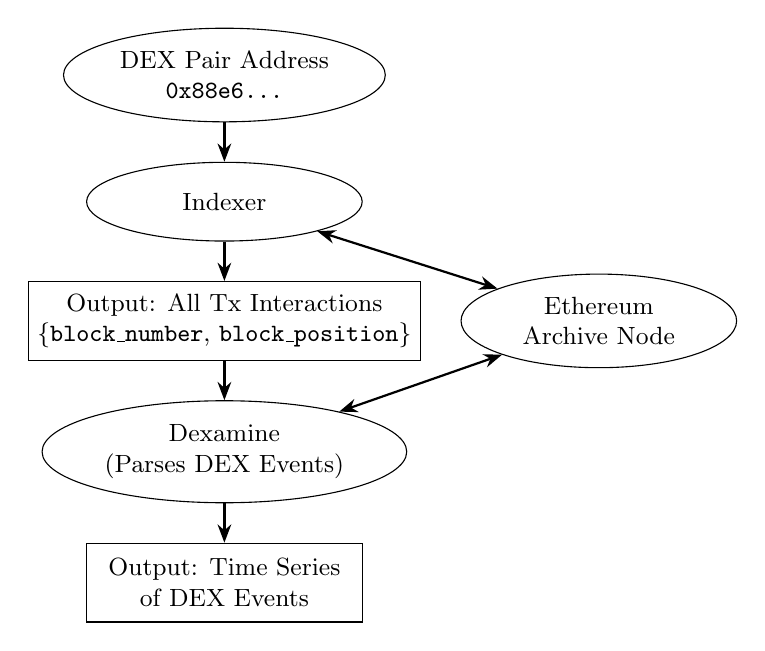
\begin{tikzpicture}[
    node distance=0.5cm and -0.5cm,
    software/.style = {ellipse, draw, align=center, minimum width=3.5cm, minimum height=1cm, font=\small},
    output/.style = {rectangle, draw, align=center, minimum width=3.5cm, minimum height=1cm, font=\small},
    arrow/.style = {->, thick, >=Stealth},
    bidirarrow/.style = {<->, thick, >=Stealth}
]

% Nodes arranged in a vertical layout
\node[software] (user) {DEX Pair Address \\ \texttt{0x88e6...}};
\node[software, below=of user] (indexer) {Indexer};
\node[output, below=of indexer] (tx_positions) {Output: All Tx Interactions \\ \{\texttt{block\_number}, \texttt{block\_position}\}};
\node[software, below=of tx_positions] (dexamine) {Dexamine \\ (Parses DEX Events)};

% Centering the Archive Node
\node[software, right=of tx_positions, xshift=1cm] (node) {Ethereum \\ Archive Node};

% Final output
\node[output, below=of dexamine] (output) {Output: Time Series \\ of DEX Events};

% Arrows
\draw[arrow] (user) -- (indexer);
\draw[arrow] (indexer) -- (tx_positions);
\draw[arrow] (tx_positions) -- (dexamine);
\draw[arrow] (dexamine) -- (output);

% Bi-directional Arrows for Archive Node
\draw[bidirarrow] (indexer) -- (node);
\draw[bidirarrow] (dexamine) -- (node);

\end{tikzpicture}

\end{document}
